\chapter{Scania ECU} \label{rtc-c300}

% The communicator contains iMX6 series processors

Scania ECU was selected as the target hardware for benchmarking the training of a machine learning model. This ECU was developed by an external system manufacturer in collaboration with Scania and is equipped with an i.MX6 series processor, specifically the MCIMX6Q-SDB, along with various on-board peripherals including CAN controllers, Ethernet, and Wi-Fi capabilities. It is worth noting that many of the configuration files for the build system and Yocto Board Support Packages (BSP) used for this specific hardware platform were not disclosed by the system manufacturer. Instead, they provided Scania with pre-built embedded Linux binaries and Software Development Kits (SDKs).

As part of the initial project objectives, there was a need to create a custom BSP layer tailored for the Scania ECU platform, which would enable the effective reconfiguration and utilization of the onboard hardware resources. To achieve this goal, a comprehensive examination of the hardware on the board was carried out. This section of the report will provide a detailed account of the activities undertaken during this effort.

\begin{figure}[h]
	\centering
	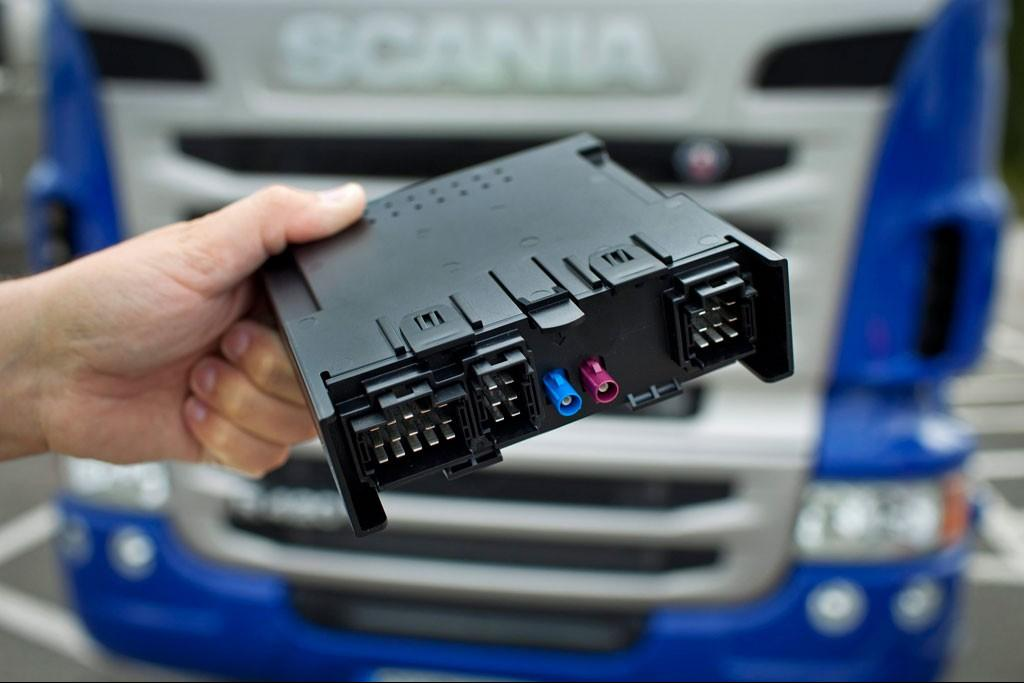
\includegraphics[scale=0.34]{c300.jpeg}
\end{figure}

\section*{Development Tools}
% (TODO: Using mfgtools on board, to collect information from bootloader.)
% (TODO: Using uuu tool in SDM mode to flash custom image.)
% (TODO: bootloader flashing using dd command)

The following methods and tools were employed to achieve our objectives, which involved configuring the hardware and flashing the necessary software components onto the Scania C300 platform.

\begin{itemize}
	\item \textit{mtd-utils}: The mtd-utils, also known as MTD (Memory Technology Device) utilities, is a set of open-source software tools for managing flash memory devices, including NAND and NOR flash memory. These utilities enable various operations like erasing, writing, and reading data on flash memory, making them essential for configuring and programming embedded systems.
	\item \textit{uuu} tool: The uuu (Universal Update Utility) is a versatile open-source tool used for flashing firmware and software onto embedded devices. It supports various hardware platforms and communication protocols, making it suitable for our flashing needs.
	\item \texttt{Serial download mode} of i.MX6 processors: This refers to the specialized mode in which the i.MX6 series processors can be placed to establish a serial communication link with a host computer. It allows for low-level programming and debugging of the processor.
	\item \texttt{SDP (Serial Download Protocol)} and \texttt{FastBoot} protocol: These are communication protocols used for transferring data between the host computer and the target hardware during the flashing process. SDP is a low-level protocol, while FastBoot is a higher-level protocol used for more advanced operations.
	\item Using \texttt{dd} to flash bootloader: The \texttt{dd} command is a versatile utility in Unix-like operating systems that can be used for copying and converting files. In the context of flashing, \texttt{dd} is often used to write bootloader images or firmware directly to storage media, such as SD cards or eMMC (embedded MultiMediaCard) devices.
\end{itemize}

% Research and experiments conducted on the Scania ECU to reverse engineering and obtain the required hardware and software information . Further, repurposing the ECU by flashing a custom operating system to benchmark the neural network applications was also attempted.

% The efforts were conducted both when the ECU started up in its usual operation and when it was booted in serial download mode.

\section*{Detailed Work and Experimental Findings}

In this section, an account of the experimental findings about the ECU is described. From understanding the hardware to the challenges faced when building a custom bootloader using the Yocto Project, this section offers a narrative of the hands-on experience and the knowledge gained through these experiments.

\subsection{Observing the Boot Up Logs and MMC Device Partitioning}

Our exploration of the Scania ECU begins with a detailed examination of the hardware, specifically focusing on the MMC (MultiMediaCard) device housed within. This vital component plays a critical role in the system's operation, as it is responsible for storage and retrieval of essential firmware and data. The \texttt{dmesg} command was used to understand the structure of the MMC (MultiMediaCard) device. This device had been partitioned into 12 distinct regions described below:

\begin{itemize}
	\item \texttt{uboot}: This partition is dedicated to the storage of the bootloader, which is crucial for the boot process.
	\item \texttt{env1} and \texttt{env2}: These partitions contain configurations for the bootloader, influencing its behavior and boot parameters. Storing these configurations separately allows for redundancy and recovery in case one configuration becomes corrupted.
	\item \texttt{eva1} and \texttt{eva2}: These partitions might be used for evaluation binaries, potentially for testing and validating different firmware or software versions.
	\item \texttt{dtb1} and \texttt{dtb2}: These partitions typically hold the device tree binaries, which provide information about the hardware configuration to the kernel.
	\item \texttt{kernel1} and \texttt{kernel2}: These regions store kernel images, each corresponding to a specific partition.
	\item \texttt{dtbupdates}: This partition may be used for device tree updates.
	\item \texttt{kernelupdate}: Similarly, this partition may be used for kernel updates.
	\item \texttt{rootfsupdate}: This region could be used for root filesystem updates, potentially for system maintenance.
\end{itemize}

\subsection{Custom Bootloader Building}

After obtaining information about the partition structure, the contents of \texttt{env1} and \texttt{env2} was downloaded using the tools in the \texttt{mtd-utils}. It was found that \texttt{env1} and \texttt{env2} contain bootloader configurations, which are essential for specifying the boot parameters, kernel command-line options, and other settings for the bootloader. The \texttt{uboot} partition, as mentioned, contains the bootloader itself. This is the software responsible for initiating the boot process, loading the kernel, and facilitating the transition from the bootloader to the kernel.

To modify the bootloader \textquotesingle s configuration, certain Linux utility programs designed for managing the bootloader were used. One such command, \texttt{fw\_setenv}, allowed us to change environment variables that influence the behaviour of the bootloader. Changing these variables can impact the boot process and system behaviour.

Based on the insights obtained from analysing partition binaries and boot-up logs, we embarked on building a custom bootloader using the Yocto Project. The U-Boot bootloader built from the Yocto Project was flashed onto the MTD partitions using APIs provided by \texttt{mtd-utils}. However, this process resulted in the board being "bricked," rendering it inoperable. Several factors could have contributed to this issue, including an incomplete or incorrect device tree structure, version mismatches between the bootloader and kernel, checksum failures, or potentially overwriting a crucial region with a larger file.

\subsubsection{Board Recovery}

The i.MX processors including the one in the Scania ECU, support a special mode known as Serial Download Mode (SDM). This mode provides a low-level interface for programming and recovering the device. In SDM, the device is in a state where it is ready to receive and execute commands provided by the host. These commands can include flashing new firmware, updating bootloader configurations, and even restoring the device to its factory state.

Following the bricking of the board, it was recovered using the board's capability to boot from SDM mode. We leveraged protocols such as SDP (Serial Download Protocol) and FastBoot, along with binaries provided by the system maker, to un-brick the board. This involved soldering the hardware, reprogramming the bootloader and potentially other firmware components to restore the system's functionality.

\subsection{Memory Layout Challenges and Absence of Board Support Packages}

Throughout these experiments, we encountered significant challenges due to the absence of board support packages (BSPs) from the system maker. BSPs typically include essential software components and configurations for a specific hardware platform, greatly simplifying the process of building and customizing the bootloader and kernel using tools like the Yocto Project.

The lack of BSPs from the system maker presented several issues

\begin{enumerate}
	\item Incomplete Information: Without BSPs, we lacked crucial information about the hardware platform, including memory layout details, required device tree configurations, and essential bootloader settings. This made it challenging to ensure compatibility between the custom bootloader built using the Yocto Project and the specific hardware of the Scania ECU.
	\item Compatibility Issues: The absence of BSPs meant that we had to make assumptions and reverse-engineer certain aspects of the hardware and software interface. This led to potential compatibility issues between the custom-built bootloader and the hardware, which, in turn, could result in bricking the board or other operational problems.
	\item Time and Resource Intensiveness: Building a bootloader without BSPs is a resource-intensive and time-consuming process. It requires extensive trial and error to ensure that the bootloader is correctly configured for the hardware.
\end{enumerate}

Addressing these challenges would have been significantly more straightforward if the system maker had provided comprehensive BSPs. These packages typically include detailed documentation and configuration files tailored to the hardware, simplifying the development and maintenance of firmware components.